\documentclass[12pt,spanish]{article}
\usepackage{graphicx}
\graphicspath{ {Graficas/}}
\usepackage[T1]{fontenc}
\usepackage[utf8]{inputenc}
\usepackage{pdfpages}
\usepackage{hyperref}
	
\usepackage{fancyhdr}
\usepackage{amssymb}
\usepackage{amsmath}
\usepackage{enumerate}
\usepackage[noend]{algpseudocode}
\usepackage{algorithm}
\usepackage[spanish]{babel}
\usepackage{vmargin}
\usepackage{subcaption}
\setpapersize{A4}
\setmargins
	{2cm}  				   % margen izquierdo
	{1.5cm}                % margen superior
	{16.5cm}               % anchura del texto
	{23.42cm}              % altura del texto
	{10pt}                 % altura de los encabezados
	{1cm}                  % espacio entre el texto y los encabezados
	{0pt}                  % altura del pie de página
	{2cm}                  % espacio entre el texto y el pie de página
	
\providecommand{\abs}[1]{\lvert#1\rvert}
\pagestyle{fancy}
\newcommand{\sectionbreak}{\clearpage}

\usepackage{xcolor}
\hypersetup{
	colorlinks,
	linkcolor={black!50!black},
	citecolor={blue!50!black},
	urlcolor={blue!80!black}
}
\rhead{Practica 3}
\lhead{Criptografía y Computación}
	
\setcounter{secnumdepth}{0} % sections are level 1

\author{
	\\\\
	
\includegraphics[scale=1]{UGR} \\
	\linebreak\\
	\Large Rafa Bailón Robles\\
	\Large Antonio Manuel Fresneda Rodríguez\\
	\Large Ismael Marín Molina\\
}

\title{\huge \textbf{Criptografía y Computación\\ Práctica 3}}

\begin{document}
	\maketitle
    \pagebreak
    \tableofcontents
    \pagebreak
 	
 	\section{Logaritmo Discreto}
 	
		\subsection{Explicación}
	 	
El objetivo en esta sección es el de resolver el problema del logaritmo discreto y ver como se comportan distintos algoritmos cuando el problema crece:
\\
Dados un primo $p$, $a$ un entero tal que $2 \leq a \leq p-2$ y $b$ otro entero $1 \leq b \leq p-1$ encontrar $x$ tal que $a^{x} \equiv b \pmod{p}$.
\\
Se han usado los siguientes algoritmos: 
\begin{itemize}
	\item\textbf{Fuerza bruta}.
	\item\textbf{Paso enano - paso gigante}.
	\item\textbf{\boldmath $\rho$ de Pollard}.
\end{itemize}
En cuanto a la ejecución de los algoritmos, se han establecido un número de iteraciones para cada uno de los algoritmos y en cada una se incrementa en dos bits el primo en el que se está trabajando. El primer primo de cada iteración tiene 5 bits.
		
		\pagebreak

		\subsection{Gráficas}

A continuación se presentan unas gráficas en las que vemos como crece el problema cuando vamos aumentando la dificultad: 
\begin{figure}[!htbp]			
	\begin{subfigure}{.5\textwidth}
		\centering
		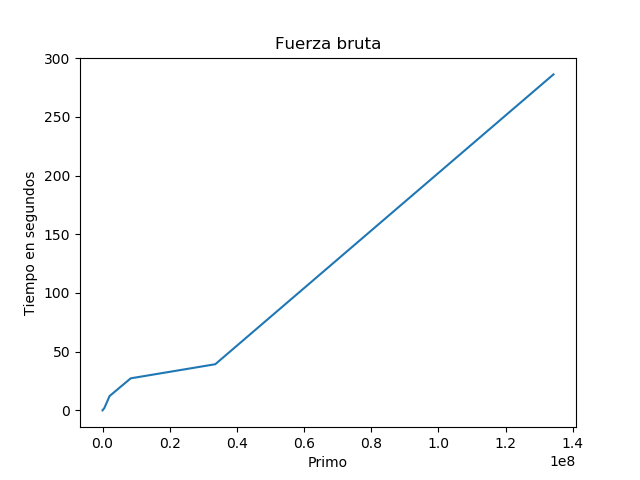
\includegraphics[width=.8\linewidth]{log_bf}
		\caption{Usando el algoritmo de fuerza bruta.}
		\label{fig:sfig11}
	\end{subfigure}
	\begin{subfigure}{.5\textwidth}
		\centering
		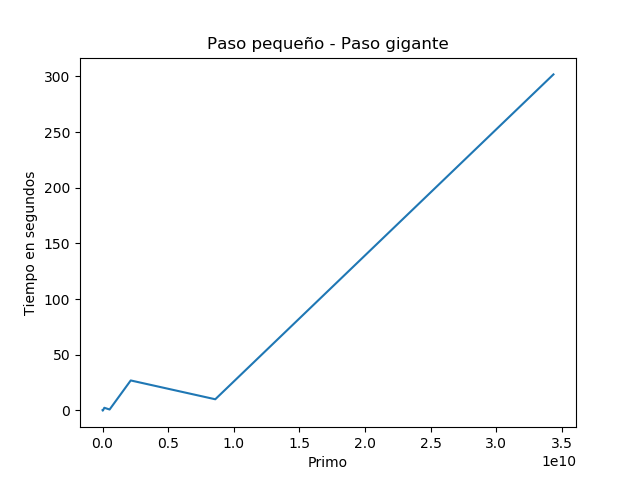
\includegraphics[width=.8\linewidth]{log_pe}
		\caption{Usando el algoritmo de paso enano - paso gigante.}
		\label{fig:sfig12}
	\end{subfigure}
	\begin{subfigure}{.5\textwidth}
		\centering
		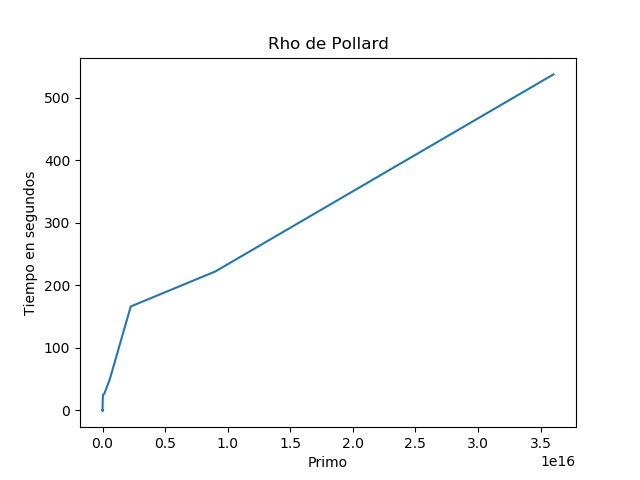
\includegraphics[width=.8\linewidth]{log_ro}
		\caption{Usando el algoritmo Rho de Pollard.}
		\label{fig:sfig13}
	\end{subfigure}
	\caption{Graficas logaritmo discreto.}
	\label{fig:fig1}
\end{figure}

		\subsection{Conclusiones}

Observando las gráficas anteriores, vemos como los distintos algoritmos que hemos usado llega un momento en el que tiempo empleado en resolver el problema se dispara.
\\
Si comparamos los tres algoritmos vemos como el de fuerza bruta ha sido el que peor se ha comportado, seguido del algoritmo de paso enano - paso gigante y el algoritmo que mejor se ha comportado ha sido el de Rho de Pollard.
\\
	
	\section{Factorizacion}
	
		\subsection{Explicacion}

El objetivo en esta sección es el de resolver el problema de la factorización y ver como se comportan distintos algoritmos cuando el problema crece. Se han usado los siguientes algoritmos: 
\begin{itemize}
	\item\textbf{Tentativa}.
	\item\textbf{Fermat}.
	\item\textbf{\boldmath $\rho$ de Pollard}.
\end{itemize}
En cuanto a la ejecución de los algoritmos, se han establecido un limite de tiempo, y probado con diferentes formas de generar los numeros compuestos para comprobar como evolucionan os tiempos según como lo generemos.
	
		\subsection{Graficas}
	
\begin{figure}[!htbp]			
	\begin{subfigure}{.5\textwidth}
		\centering
		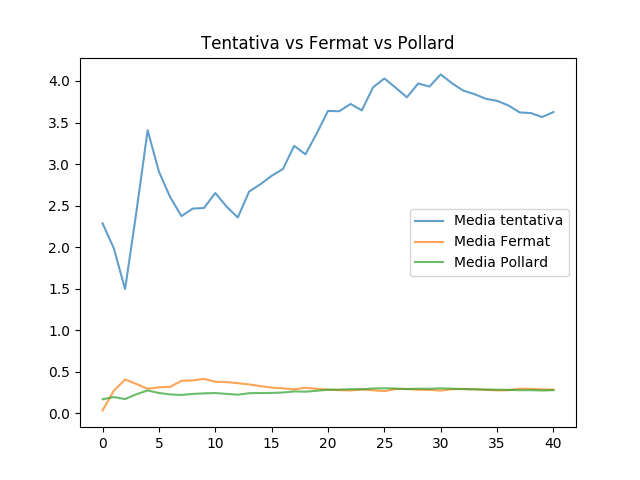
\includegraphics[width=.8\linewidth]{EvolucionMedias}
		\caption{Compuestos aleatorios}
		\label{fig:sfig21}
	\end{subfigure}%
	\begin{subfigure}{.5\textwidth}
		\centering
		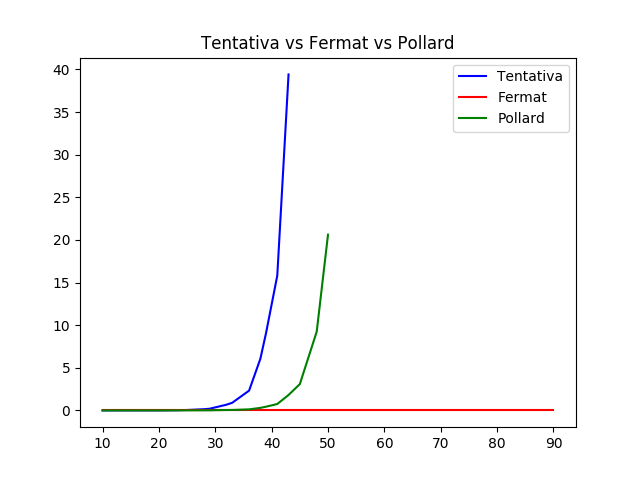
\includegraphics[width=.8\linewidth]{NearComp}
		\caption{Compuestos de primos cercanos}
		\label{fig:sfig22}
	\end{subfigure}
	\begin{subfigure}{.5\textwidth}
		\centering
		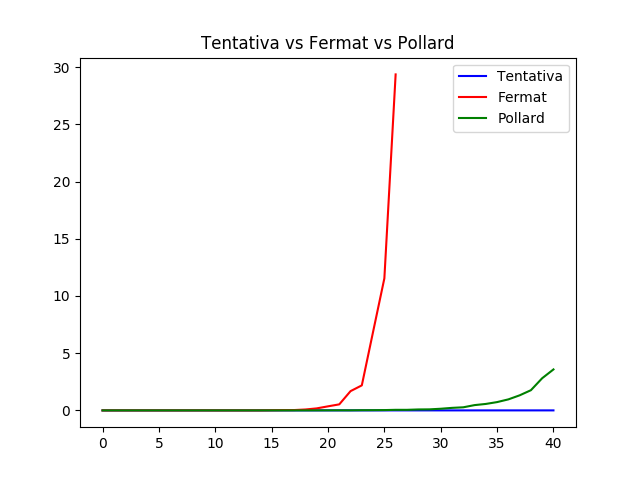
\includegraphics[width=.8\linewidth]{VentajaTentativa}
		\caption{Compuestos con un primo pequeño}
		\label{fig:sfig23}
	\end{subfigure}
	\caption{Graficas factorizacion.}
	\label{fig:fig2}
\end{figure}
		
	\section{Raíces Cuadradas Modulares}
	
		\subsection{Explicación}
		
Dado un número entero $a$ y un primo impar $p$, el algoritmo calcula un número $r$ que cumpla que $x^2 \equiv a \mod{p}$ o, lo que es lo mismo, que $r^2 mod p = a$.
\\
Primeramente debemos saber si el número tiene, o no, raíz cuadrada modular. Para ello tenemos el símbolo de Legendre y el símbolo de Jacobi. El primero es un caso particular del segundo, que es más general. Si partimos del símbolo de Jacobi, siendo $p$ un número primo impar, tenemos que el algoritmo devolverá 1 como resultado si existe la raíz. El símbolo de Jacobi garantiza su existencia siempre que $p$ sea primo impar, ya que, el algoritmo, acepta que $p$ sea un número impar cualquiera pero, en ese caso, no garantiza que exista una raíz cuadrada modular.
\\
Apoyándonos en el símbolo de Jacobi, se construye el algoritmo de Tonelli. Si Jacobi nos dice si existe la raíz, Tonelli calcula dicha raíz $r$. Por tanto, el resultado de su ejecución, dados un número entero $a$ y un primo impar $p$, es un $r$ que cumple que $r^2 mod p = a$.

		\subsection{Gráficas}
		
A continuación podemos ver la gráfica de la ejecución del algoritmo de Tonelli. El tiempo de ejecución está en milisegundos ya que el algoritmo es bastante eficiente incluso con números muy grandes (en las pruebas se ha llegado a usar $a$ y $p$ de 300 cifras). En lugar de poner los números primos, dado su tamaño, en la gráfica aparecen el número de cifras que lo componen.
\begin{figure}[!htbp]			
		\centering
		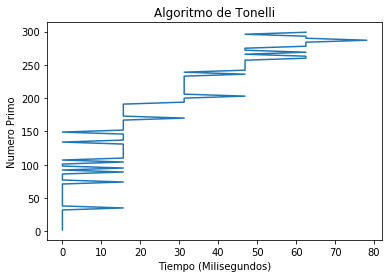
\includegraphics[width=.8\linewidth]{raiz_cuadrada}
		\caption{Gráfica - Raíz Cuadrada Modular}
	\label{fig:fig3}
\end{figure}
		
		\subsection{Conclusiones}
		
El algoritmo de Tonelli responde bastante bien incluso con números muy grandes. El tiempo en milisegundos en prueba de ello. Se han incluido mensajes para comprobar, además, que los resultados son correctos en todos los casos. Las pruebas expuestas en la gráfica constan de 100 ejecuciones del algoritmo, incrementando cada vez el tamaño de los valores $a$ y $p$.		
		
\end{document}